\documentclass[10pt, conference, letterpaper]{IEEEtran}

\usepackage{graphicx}
\usepackage{amsmath}
\usepackage{amssymb}
\usepackage{booktabs}
\usepackage{cite}
\usepackage{subcaption}
\usepackage{algorithm}
\usepackage{algpseudocode}
\usepackage{url}

\graphicspath{{./figures/}}

\IEEEoverridecommandlockouts

\begin{document}

\title{Weather Image Classification with Engineered Features and Support Vector Machines}
\author{Alexandru Mihailescu\thanks{Work done for the course of Computer Vision, taught by Prof. Pietro Zanuttigh at the University of Padua.}}

\maketitle

\begin{abstract}
This paper presents a classical computer vision pipeline for multi-class weather image classification, built without any deep learning component. The objective is to recognise four weather conditions (cloudy, rainy, shine, sunrise) in the Multi-class Weather Dataset (MWD). The approach engineers a compact colour-oriented descriptor for each image, combining BGR channel histograms, per-channel contrast statistics, dominant colours extracted by k-means, and the HSV histograms of a Difference-of-Gaussian version of the image. The 1562-dimensional descriptor is projected onto 200 principal components and fed to a support vector machine whose hyperparameters are selected by grid search. The feature set itself was assembled empirically, one candidate at a time, with the test score of the fitted SVM as the selection criterion. The resulting classifier reaches 96.04\% accuracy on the MWD test split. The same descriptor and the same model class were then carried over to the Adverse Conditions Dataset with Correspondences (ACDC), a five-class driving dataset whose classes are far less separable in colour space. ACDC has a different class set, so the descriptor transfers unchanged while the PCA and the SVM are refitted on the ACDC training split, and the pipeline reaches 90.6\% test accuracy there. That second experiment is the more informative of the two: it puts a number on what a colour-specialised feature set costs when the data distribution changes, and it locates the loss precisely, in the mutual confusion of rain, snow and fog.
\end{abstract}

\section{Introduction}

The task is to assign a weather label to a single still image. The solution is built from scratch out of classical computer vision primitives: no pretrained network, no learned feature extractor, no end-to-end training. Every dimension of the descriptor is something a human chose to compute.

That constraint is the point of the exercise. It forces the design question into the open: which measurable property of an image separates a rainy scene from a cloudy one? For the four MWD classes the honest answer is colour, plus a little texture. Sunrise images are dominated by warm hues, cloudy images by a narrow band of greys, shine images by high-saturation blues. Rain is the hard class, because a rainy scene is, in colour terms, a slightly desaturated cloudy scene.

The pipeline is therefore built around colour descriptors, with a Difference-of-Gaussian (DoG) term added to capture the high-frequency structure that rain and cloud edges produce. Features are pushed through a principal component analysis and classified by a support vector machine \cite{cortes1995svm}. The individual operators are all standard. The contribution is the empirical loop used to select them and the cross-dataset test used to check whether the result means anything outside the dataset it was tuned on.

\section{Data}

\subsection{MWD}

The Multi-class Weather Dataset \cite{ajayi2018mwd} contains 1125 images in four classes: cloudy, rain, shine, sunrise. The images are web-sourced, of heterogeneous resolution and quality, and the classes are unbalanced. The dataset ships in a training and a test directory, with 847 and 278 images respectively.

Two of the training images could not be decoded by the OpenCV \cite{bradski2000opencv} \texttt{imread} function, which returns an uninitialised variable rather than raising. Those two are skipped at load time. The usable data is therefore 845 training images and 278 test images, 1123 in total. The test split contains 75 cloudy, 52 rain, 62 shine and 89 sunrise images.

The test split is used as the model selection criterion throughout the feature engineering loop described in Section~\ref{sec:features}. This is the standard caveat that applies to any empirical feature search: the final test accuracy is optimistically biased, because the test split guided the choices. The cross-dataset experiment in Section~\ref{sec:acdc} is the check against that bias.

\subsection{ACDC}
\label{sec:acdc-data}

The Adverse Conditions Dataset with Correspondences \cite{sakaridis2021acdc} is a driving dataset built for semantic segmentation under adverse conditions. Its images are labelled with five conditions: clear, fog, night, rain, snow. Used here as a classification benchmark, it provides 1000 training images and 500 test images, balanced at 100 test images per class.

ACDC is a deliberately hostile target for this pipeline. All of its images come from a vehicle-mounted camera, so they share a composition, a horizon line and a road surface. The classes are distinguished by weather, not by scene type, and several of them (rain, snow, fog) share a washed-out low-saturation palette. A descriptor built to separate a sunrise from a blue sky has no obvious reason to work here.

\section{Feature Engineering}
\label{sec:features}

\subsection{The empirical loop}

Feature selection was driven by measurement rather than by theory. Starting from a single descriptor family, candidate features were added and removed one at a time, the SVM was refitted, and the change in test accuracy decided whether the candidate stayed. Fig.~\ref{fig:iterations} records the whole sequence: each column is one feature configuration, and the bottom row is the test accuracy it produced.

\begin{figure}[t]
\centering
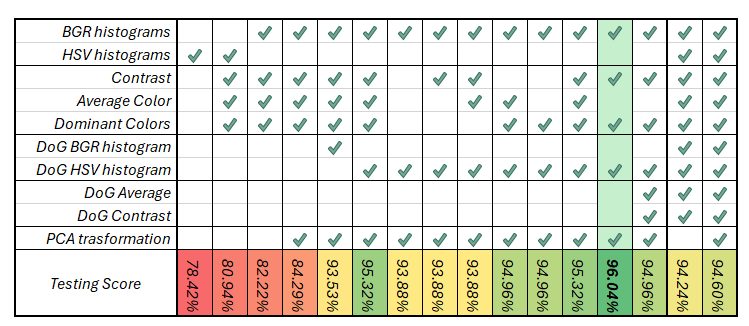
\includegraphics[width=\columnwidth]{feature-selection-iterations.png}
\caption{Feature configurations tested and the resulting MWD test accuracy. Each column is one iteration of the loop. The highlighted column is the configuration that was kept.}
\label{fig:iterations}
\end{figure}

Four results from that loop are worth stating explicitly.

\textbf{BGR beat HSV.} The loop started with HSV histograms, on the assumption that a perceptual colour space carries more usable signal than raw sensor channels. It does not, at least not here: swapping HSV histograms for BGR histograms moved the score from 78.42\% to 82.22\%. The assumption was wrong and the measurement said so.

\textbf{DoG histograms were worth roughly 9 points.} Adding the histograms of the Difference-of-Gaussian image raised the score by about nine percentage points, the single largest jump in the table. The DoG was computed on the colour image rather than on a greyscale version, deliberately. Reducing a colour-driven classification problem to greyscale before extracting the edge response throws away exactly the information the rest of the pipeline is built on, and the SVM proved able to use what was left in.

\textbf{HSV beat BGR for the DoG term.} The opposite of the raw-image result. Fig.~\ref{fig:dog} shows why. The three BGR channels of the DoG image are nearly identical, so the BGR histogram triples one signal and carries almost nothing else. The HSV histogram of the same image separates that shared component into the lightness channel and exposes hue and saturation structure that BGR does not represent. Switching the DoG term from BGR to HSV added a further two points.

\begin{figure}[t]
\centering
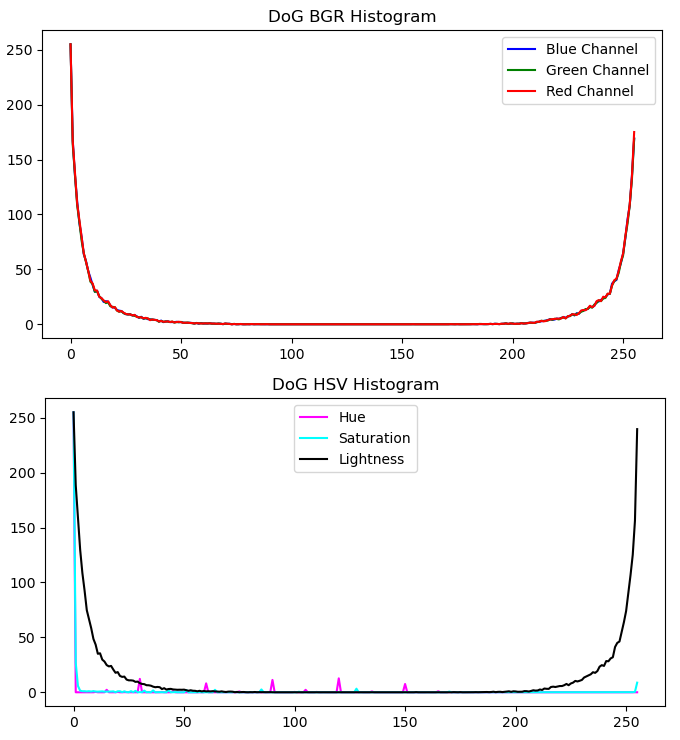
\includegraphics[width=\columnwidth]{dog-histograms-comparison.png}
\caption{BGR and HSV histograms of the Difference-of-Gaussian of the same training image. The three BGR channels are almost coincident and duplicate the HSV lightness channel; the hue and saturation channels carry the information that BGR does not.}
\label{fig:dog}
\end{figure}

\textbf{Average colour hurt.} Contrast, average colour and dominant colours together contributed almost two points. Removing average colour while keeping contrast and dominant colours contributed more. The average colour of an image is a coarse summary of information the histograms and the dominant colours already carry at higher resolution, and PCA did not eliminate the redundancy. More features are not more information.

Adding DoG average colour and DoG contrast on top of the retained set reduced the score, as did the final control run using every extractable feature at once, with and without PCA. Both outcomes are consistent with the average-colour result.

\subsection{The retained descriptor}

The configuration that was kept is listed in Table~\ref{tab:features}. All components are z-normalised before concatenation.

\begin{table}[t]
\centering
\caption{The retained feature set. Dimensions per image.}
\label{tab:features}
\begin{tabular}{lr}
\toprule
Component & Dim. \\
\midrule
BGR histograms (3 channels $\times$ 256 bins)         & 768 \\
Contrast (per-channel mean and standard deviation)    & 6 \\
Dominant colours (6 k-means centroids in RGB)         & 18 \\
DoG HSV histograms (3 channels $\times$ 256 bins)     & 768 \\
Array initialisation padding                          & 2 \\
\midrule
Total                                                 & 1562 \\
After PCA                                             & 200 \\
\bottomrule
\end{tabular}
\end{table}

\textbf{Histograms.} Per-channel 256-bin histograms over the full intensity range, z-normalised so that images of different sizes and exposures are comparable.

\textbf{Contrast.} The per-channel mean and standard deviation of the image, six numbers, z-normalised.

\textbf{Dominant colours.} The image is downsampled to $100 \times 100$ by nearest-neighbour interpolation, then k-means with $k=6$ is run on the pixels. The six centroids are sorted by cluster population and flattened, giving 18 numbers. The cluster populations themselves were tested as features and dropped. The downsampling exists to make k-means affordable across the whole dataset; feature extraction over the training split takes about 54 seconds as a result.

\textbf{Difference of Gaussian.} The difference of two Gaussian blurs of the colour image, with $1 \times 1$ and $3 \times 3$ kernels. The result is converted to HSV and histogrammed as above.

The two padding dimensions are a harmless artefact of how the feature vector is initialised in code: they are constant across every image and are annihilated by the PCA projection.

\subsection{Dimensionality reduction}

At the point in the loop where PCA was introduced, the descriptor was 797-dimensional and growing with every candidate feature. PCA was fitted with 200 components, a value chosen by the same empirical procedure: it is the smallest count found that did not degrade the SVM. The final 1562-dimensional descriptor is therefore projected to 200 dimensions, a compression of roughly 8:1. PCA is fitted on the training split only, and the same fitted transform is applied to the test split.

The reduction improved the score slightly, which is the expected behaviour when a high-dimensional descriptor contains correlated and near-constant directions, as this one does by construction.

\section{Classifier}

The classifier is a support vector machine. Hyperparameters are chosen by exhaustive grid search with cross-validation over

\begin{itemize}
  \item $C \in \{0.01,\ 0.1,\ 1,\ 10,\ 100\}$,
  \item $\gamma \in \{0.001,\ 0.1,\ 1\}$,
  \item kernel $\in \{\text{linear},\ \text{RBF},\ \text{polynomial}\}$,
\end{itemize}

evaluated in parallel across all available cores. The selected configuration is an RBF kernel with $C = 100$ and $\gamma = 0.001$: a wide kernel with a hard margin, which is what a 200-dimensional space with well-separated class clusters should be expected to want.

The fitted PCA and SVM are serialised to disk with joblib, so the model can be reloaded and used for inference without repeating the grid search.

\section{Results}

\subsection{MWD}

The final classifier reaches \textbf{96.04\% accuracy} on the 278 held-out MWD test images, with 100\% on the training split. Fig.~\ref{fig:cm-mwd} gives both confusion matrices.

\begin{figure}[t]
\centering
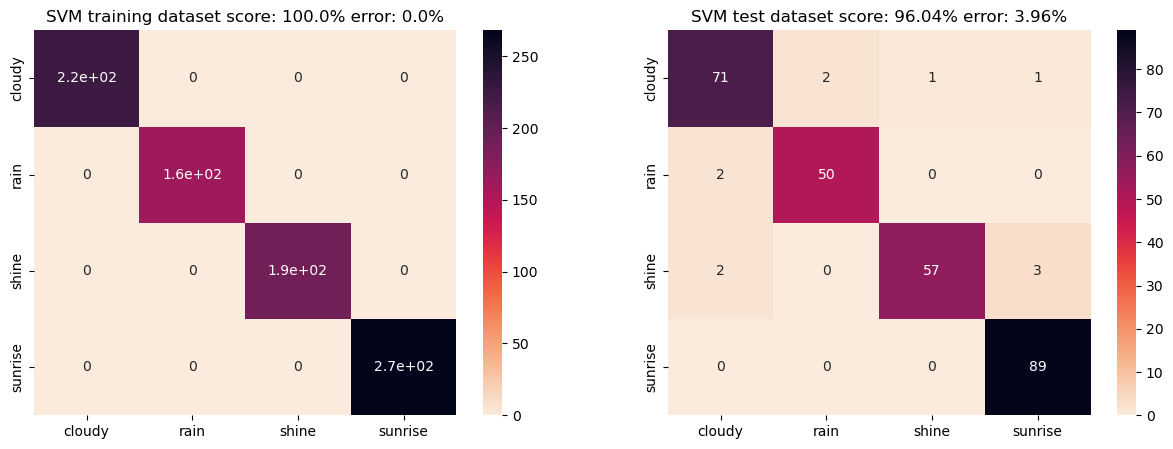
\includegraphics[width=\columnwidth]{confusion-matrix-mwd.png}
\caption{Confusion matrices on MWD, training split (left) and test split (right).}
\label{fig:cm-mwd}
\end{figure}

The gap between the training and the test score is 3.96 points. That is consistent with mild overfitting, but a saturated training score on 845 examples in a 200-dimensional space with a hard-margin SVM is close to unavoidable, and a four-point gap is not by itself evidence of a broken model.

The eleven test errors are structured:

\begin{itemize}
  \item \textbf{Cloudy against rain} (2 + 2 errors, symmetric). A rainy scene without visible precipitation streaks is a cloudy scene. The DoG term is what separates them at all.
  \item \textbf{Shine against sunrise} (3 errors) and \textbf{shine against cloudy} (2 errors). Both are lighting-condition confusions between classes that overlap in hue.
  \item \textbf{Sunrise} was never misclassified. Its colour signature, warm hues at low overall lightness, is the most distinctive of the four and the descriptor captures it cleanly.
\end{itemize}

Fig.~\ref{fig:correct} and Fig.~\ref{fig:wrong} show representative correct and incorrect predictions. The failures are not silly. The misclassified cloudy image contains a bright sky region typical of shine; the misclassified rain image is a close-up of an umbrella against out-of-focus green foliage, with none of the global colour statistics of a rainy street scene; the misclassified shine image is a backlit sun through palm trees, whose dominant colours are the dark silhouettes.

\begin{figure}[t]
\centering

\includegraphics[width=\columnwidth]{mwd-correct-classifications.png}
\caption{Correct classifications on the MWD test split, one per class.}
\label{fig:correct}
\end{figure}

\begin{figure}[t]
\centering

\includegraphics[width=\columnwidth]{mwd-misclassifications.png}
\caption{Misclassifications on the MWD test split. No misclassified sunrise image exists in the test split.}
\label{fig:wrong}
\end{figure}

\subsection{Cross-dataset transfer to ACDC}
\label{sec:acdc}

The interesting experiment is the second one. ACDC labels its images with a different set of weather conditions, so the MWD classifier cannot be scored on it directly. What is carried over is the descriptor: the feature extraction code was applied to ACDC unchanged, and a model of the same class was then fitted from scratch on the ACDC training split under the same grid search, with the PCA refitted on that split as well. Nothing about the descriptor was retuned for the new data. The quantity being measured is what a feature set tuned on one dataset is worth on another, not whether a trained classifier survives a distribution shift.

The answer is \textbf{90.6\% test accuracy} over 500 balanced test images, against 100\% on the training split. Fig.~\ref{fig:cm-acdc} gives the matrices.

\begin{figure}[t]
\centering
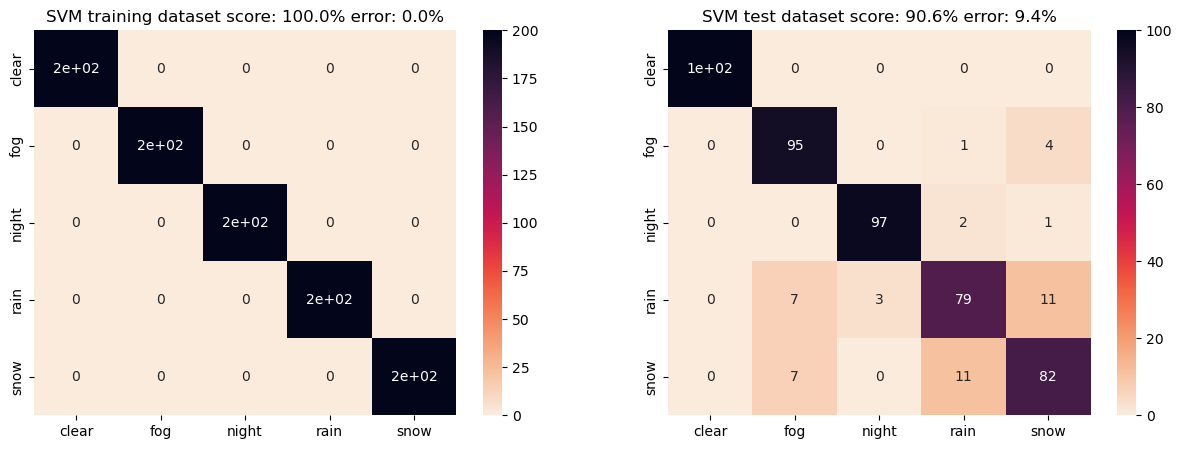
\includegraphics[width=\columnwidth]{confusion-matrix-acdc.png}
\caption{Confusion matrices on ACDC, training split (left) and test split (right). Five classes: clear, fog, night, rain, snow.}
\label{fig:cm-acdc}
\end{figure}

Three things follow from that number.

\textbf{The descriptor transfers, at a measurable price.} A colour-and-DoG feature set designed for four web-scraped weather classes still separates five driving-scene conditions at 90.6\%, on a harder five-way problem with a chance level of 20\%. That is a real result.

\textbf{The price is paid exactly where colour stops separating the classes.} The per-class accuracies are clear 100\%, night 97\%, fog 95\%, snow 82\%, rain 79\%. Clear and night are trivially separable by global lightness and hue and the classifier gets them essentially for free. The entire loss is concentrated in rain and snow, which confuse each other 22 times out of 200, and in the leakage of both of them into fog, which accounts for 14 further errors. Rain, snow and fog under an overcast sky produce nearly the same desaturated grey colour distribution. The descriptor has nothing left to say about them.

\textbf{The generalisation gap widened.} 9.4 points on ACDC against 3.96 on MWD, with a saturated training score in both cases. The model class is the same and the fitting procedure is the same, so the extra gap is attributable to the descriptor being a worse fit for the data, not to the SVM.

\begin{table}[t]
\centering
\caption{Summary. Test accuracy on both datasets.}
\label{tab:summary}
\begin{tabular}{lrrrr}
\toprule
Dataset & Classes & Train & Test & Test acc. \\
\midrule
MWD  & 4 & 845  & 278 & 96.04\% \\
ACDC & 5 & 1000 & 500 & 90.6\% \\
\bottomrule
\end{tabular}
\end{table}

\subsection{Run-to-run variance}

The dominant colour extraction uses k-means with random initial centroids and no fixed seed, so the descriptor is not deterministic across runs. Refitting the whole pipeline end to end therefore does not reproduce 96.04\% exactly: a refit of the shipped notebook scores 94.6\% on the same test split, 1.44 points below. That is the correct order of magnitude for the effect, since 18 of the 1562 dimensions are stochastic. The 96.04\% figure belongs to the fitted model serialised with this work, and is reproducible by loading that model rather than by refitting it. Seeding the k-means initialisation would remove the variance and should be done.

\section{Discussion}

\subsection{What the cross-dataset test shows}

Reporting the accuracy of a model on the dataset whose test split guided its own feature selection is close to circular. The ACDC experiment breaks that circle, and the shape of its failure is the actual finding of this work.

The feature set encodes a specific hypothesis: that weather is visible in the global colour statistics of an image. On MWD that hypothesis is nearly correct, because the four MWD classes differ in colour by construction, and the classifier is rewarded with 96\%. On ACDC the hypothesis is correct for two classes (clear, night, both separable by lightness), partially correct for one (fog, which has a distinctive low-contrast signature), and wrong for two (rain and snow, which under an overcast sky share a palette). The accuracy drops by precisely the amount those two classes contribute.

That is a clean result about the feature set, obtained only because the feature set was moved to data it was not designed for. It is worth more than the headline MWD number.

\subsection{Where the next gain is}

The failure mode points directly at the fix. Rain and snow differ in colour, but the difference is spatially localised: the sky is the same in both, while the ground in a snow scene is dominated by white and the ground in a rain scene is not. A global histogram over the whole image averages that distinction away.

The remedy is semantic segmentation of the scene into ground and sky, followed by the same colour analysis applied per region. That would recover exactly the signal the global descriptor destroys, and sky-region colour analysis would in addition support finer distinctions within a single weather class, for instance the time of day.

\subsection{Limitations}

\begin{itemize}
  \item The MWD test split was used for feature selection, so the 96.04\% figure is optimistically biased. A three-way split would have been the correct protocol.
  \item The pipeline is deliberately colour-first. It has no texture descriptor beyond the DoG histograms and no spatial structure whatsoever, since a histogram discards where in the image a colour occurred.
  \item The dominant colour extraction is unseeded, which makes the pipeline non-deterministic (Section V-C).
  \item The class balance of MWD is not corrected for, and accuracy is reported unweighted.
\end{itemize}

\section{Conclusion}

A hand-engineered colour descriptor of 1562 dimensions, reduced to 200 principal components and classified by an RBF support vector machine, reaches 96.04\% test accuracy on four-class weather classification in MWD. No learned features and no neural network are involved.

The feature set was assembled by measurement, and the measurements contradicted the initial intuitions twice: BGR histograms beat HSV on the raw image while HSV beat BGR on the DoG image, and adding average colour to a descriptor that already contained histograms and dominant colours made the classifier worse.

Carried over to ACDC with the descriptor unmodified and the model refitted on ACDC's own training split, the same pipeline reaches 90.6\% on a harder five-class problem and loses almost all of its accuracy on exactly the two classes (rain and snow) that a global colour statistic cannot distinguish. That is the honest measure of what this descriptor is: a very good weather classifier for datasets whose classes differ in colour, and a mediocre one for datasets whose classes do not. Region-wise colour analysis after semantic segmentation is the obvious next step, and the ACDC confusion matrix says exactly how much it would be worth.

\bibliographystyle{IEEEtran}
\bibliography{biblio}

\end{document}
